\begin{figure}[hbt!]
\centering
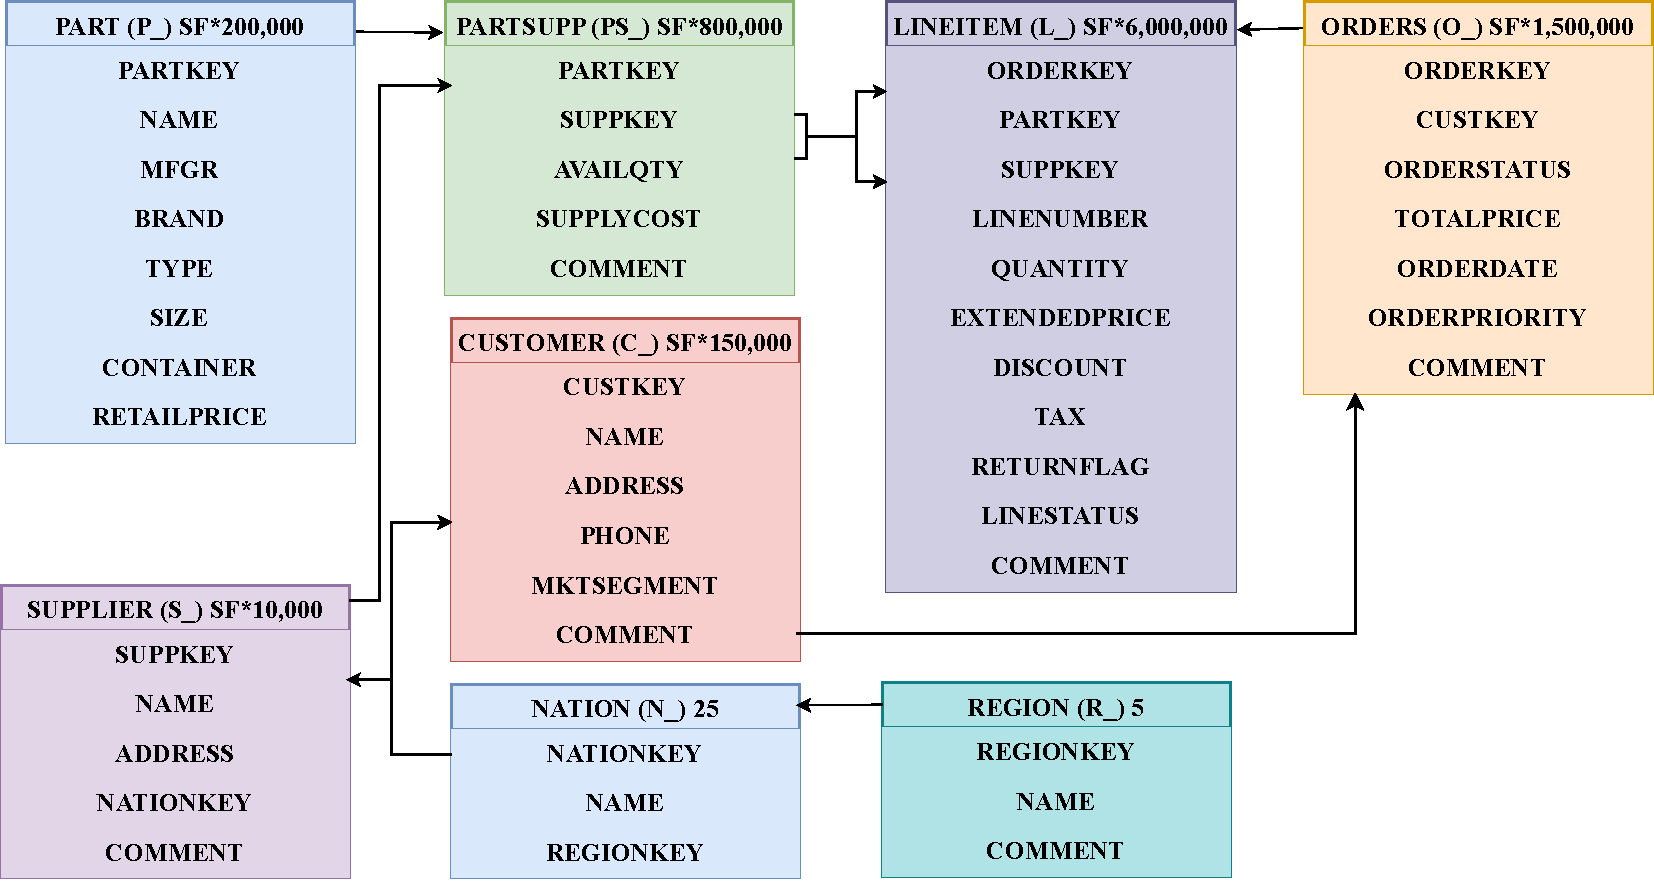
\includegraphics[width=1.0\linewidth]{img/TPCH.pdf}
\caption[The TPC-H schema]{The TPC-H schema. The parentheses following each table name contain the prefix of the column names for that table. The number/formula beside each table name represents the cardinality (number of rows) of the table. Some are factored by \acrshort{sf} to obtain the chosen database size. The cardinality for the LINEITEM table is approximate.~\cite{noauthor_tpc-homepage_2024}}
\label{fig:tpch-schema}
\end{figure}